\chapter{Consistency of estimating-equation M estimators.}

\begin{figure}[H]
\centering
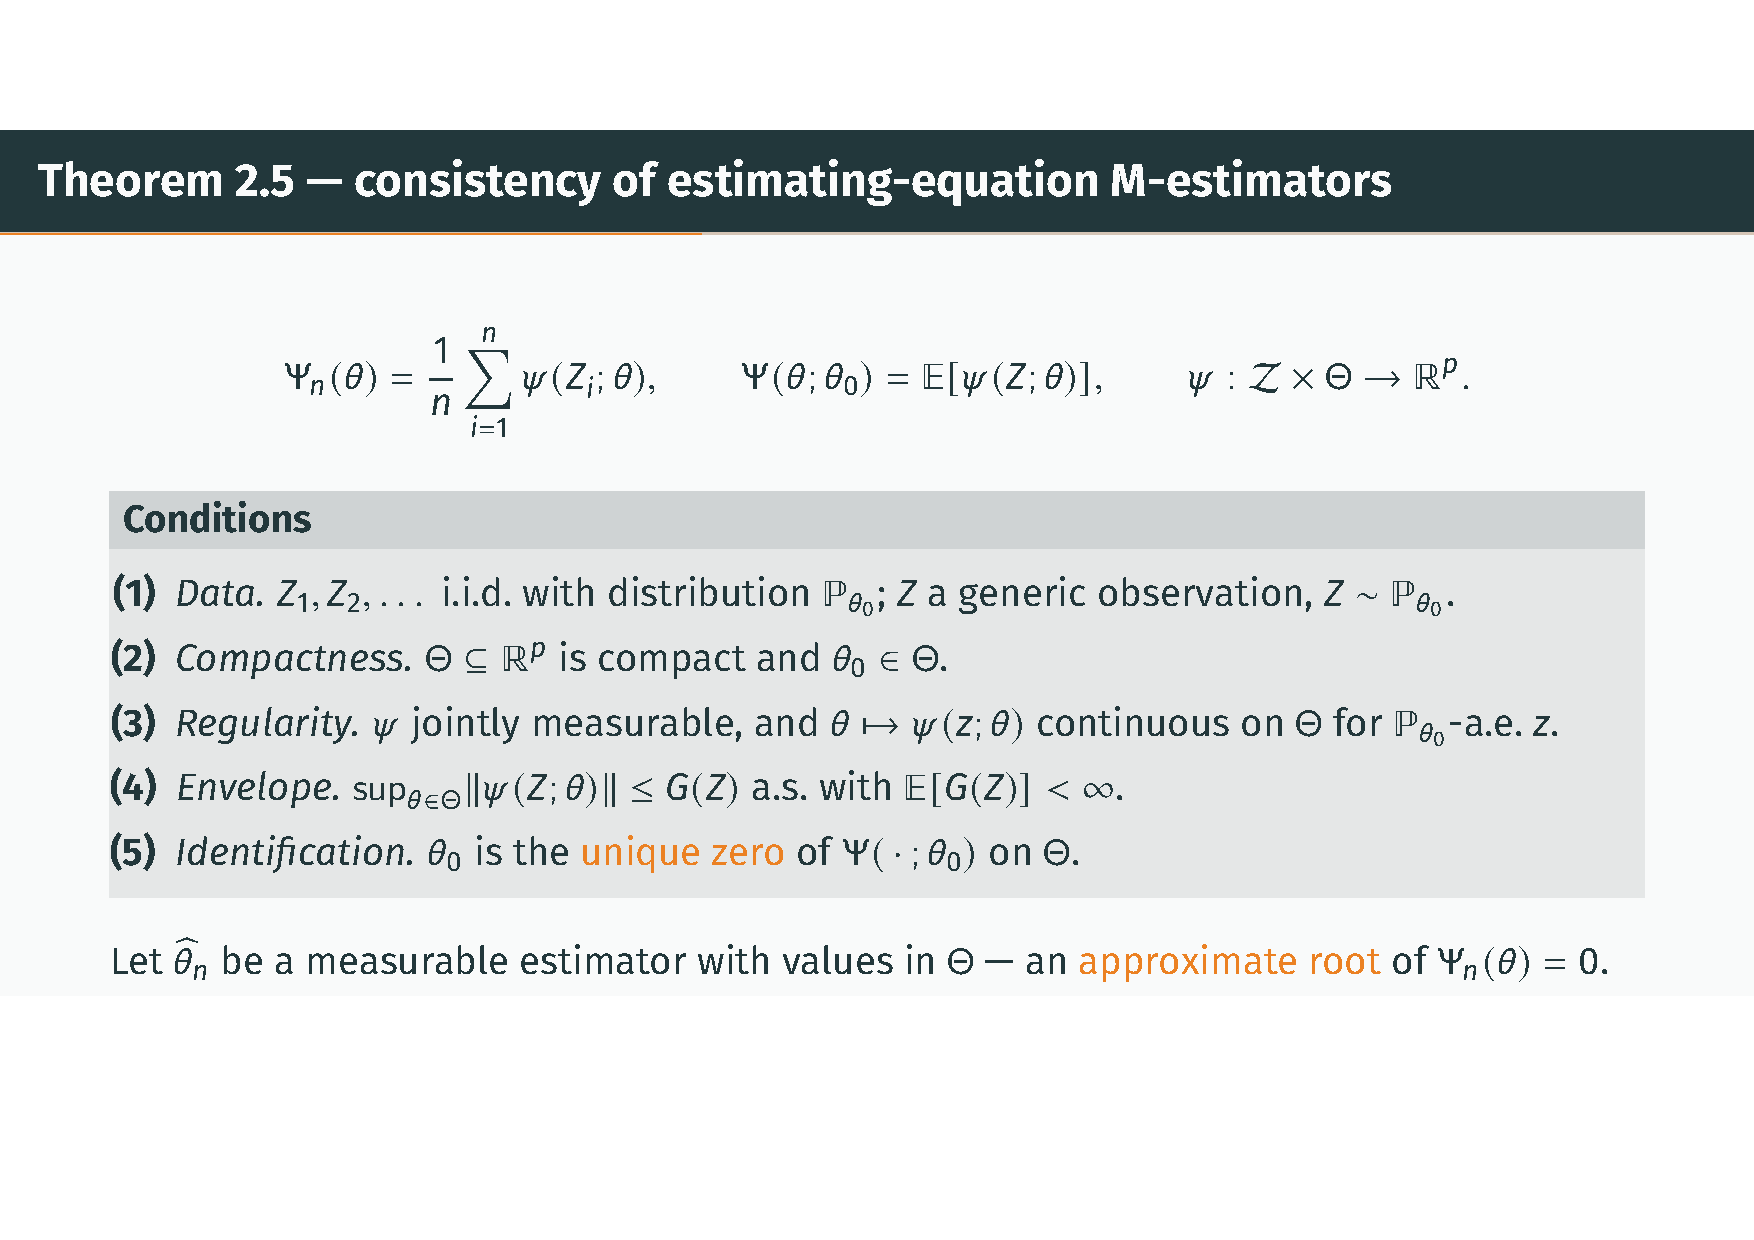
\includegraphics[width=\textwidth]{figures/Consistency-1.pdf}
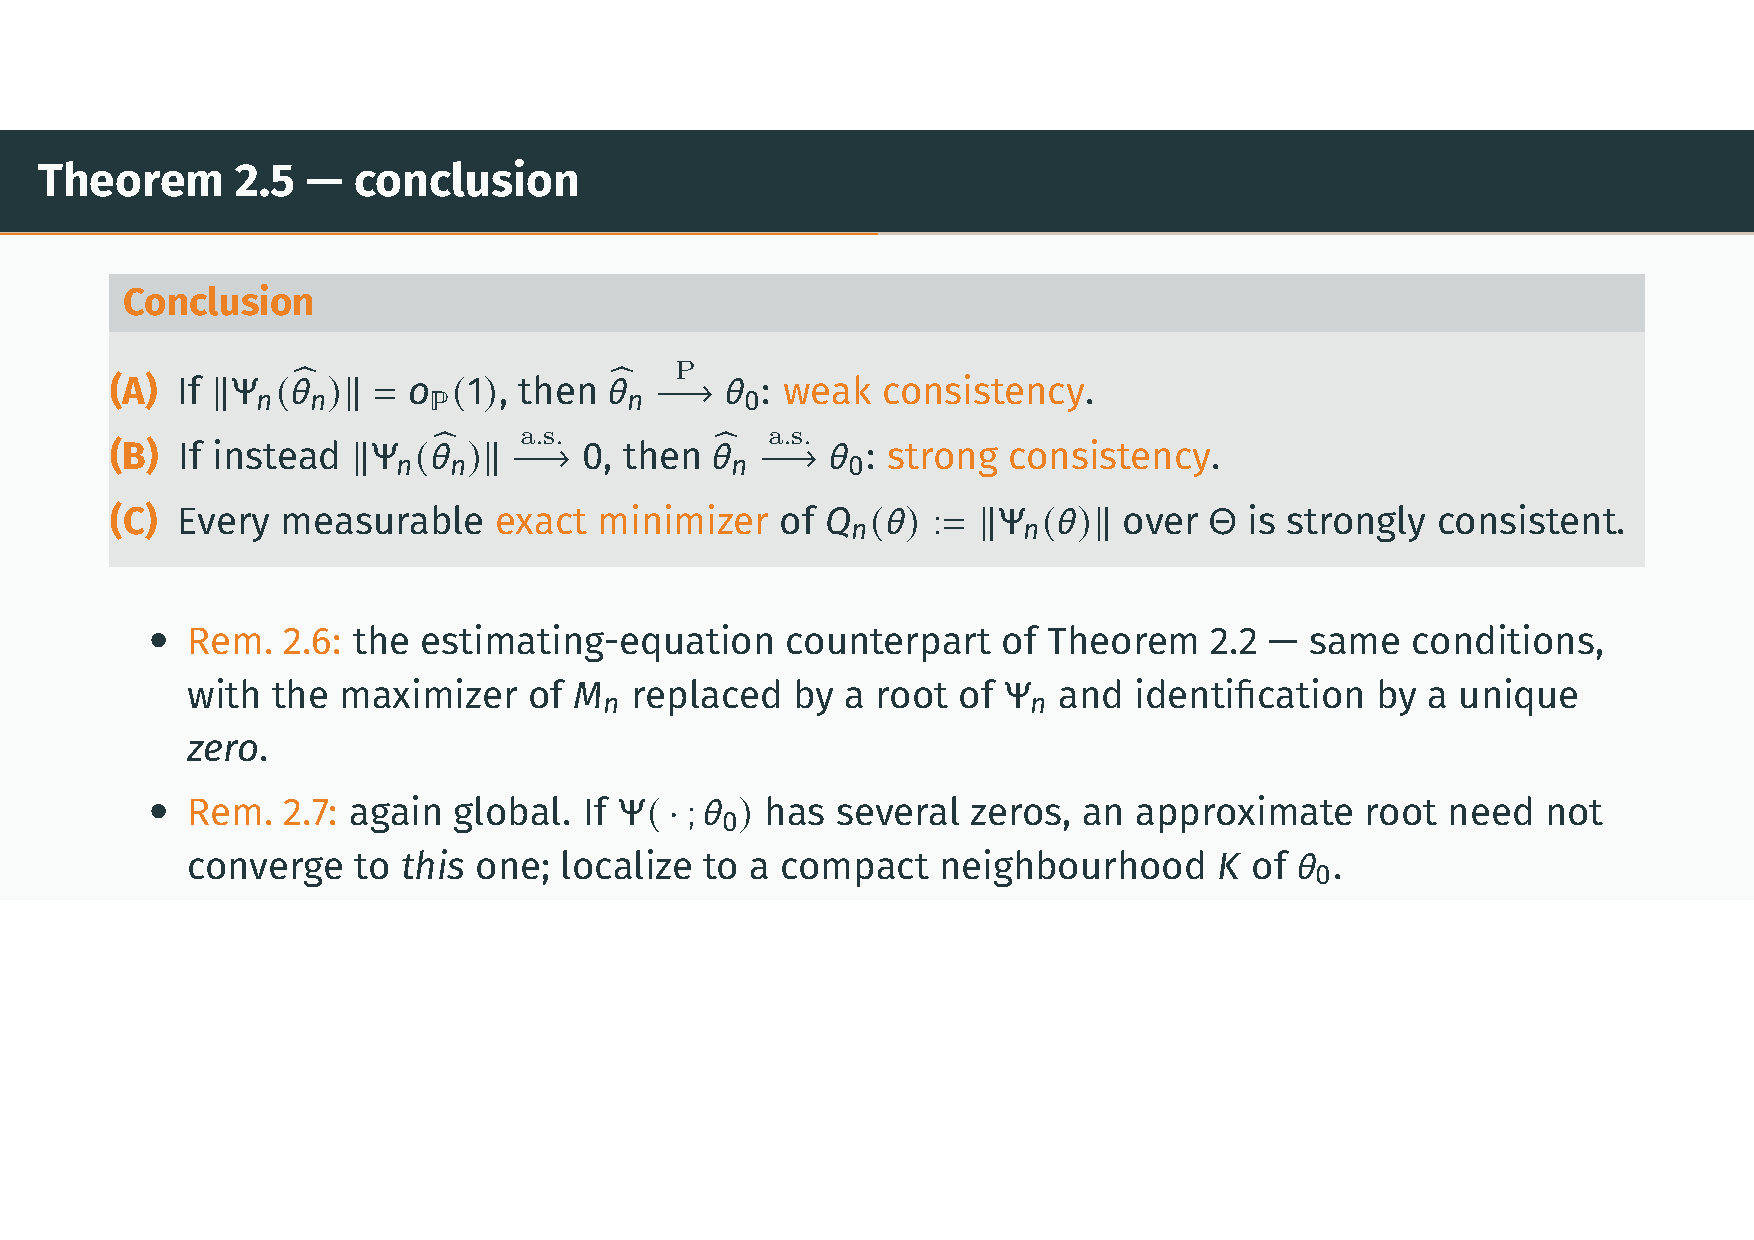
\includegraphics[width=\textwidth]{figures/Consistency-2.pdf}
\end{figure}
\noindent\textbf{Comments:}

$\what{\theta}_n$ denotes a root of the estimating equation $\Psi_n (\theta) = 0$.
Note that the regularity and envelope assumptions gives a uniform law of large numbers: 
\begin{lemma*}[2.1 (A uniform law of large numbers) (ULLN)]
  Assume \textbf{(3)} and \textbf{(4)}. Given data from \textbf{(1)} we have:
  \[ 
    \sup_{\theta \in \Theta} \left\| \frac{1}{n} \sum_{i=1}^{n} g(Z_i;\theta) - \E[g(Z;\theta)]
    \right\|
    \xrightarrow[n \to \infty ]{a.s.} 0
  .\]
\end{lemma*}
\global\def\lastproofcolor{theorembordercolor} % needed since no theorem is used here
\begin{proof}[of Theorem 2.5]

  \begin{description}
   \item []
  \item[Continuity of  $\Psi (\cdot, \theta_0).$] 
  \end{description}
  By the \textbf{(3)}, \textbf{(4)} and dominated convergence:
  \[ 
    \E\left[\sup_{\theta \in \Theta} \| \Psi(z;\theta)\| \right] \le \E[G(Z)] < \infty 
  ,\]
  thus $\theta \mapsto \Psi(\theta;\theta_0)$ is continuous (on $\Theta$).
  \begin{description}
  \item[Uniform convergence of $\Psi_n$] 
  \end{description}
  By ULLN (with $g = \Psi_n$): 
  \[ 
  \Delta_n := \sup_{\theta \in \Theta} \| \Psi_n(\theta) -  \Psi(\theta;\theta_0) \| \xrightarrow[n
  \to \infty ]{a.s.} 0  \implies \Delta_n \xrightarrow[n \to \infty ]{\P} 0
  .\]

  \begin{description}
  \item[Weak consistency] 
  \end{description}
  Assume $\| \Psi_n (\what{\theta}_n)\| = o_{\P}(1)$.
  Fix $\epsilon > 0$ and let $K_{\epsilon} = \{ \theta \in \Theta : \| \theta -  \theta_0 \| \ge
  \epsilon \}$. 

  \begin{itemize}
  \item  Assume $K_{\epsilon}$ is empty.

   Then all $\theta \in \Theta$ satisfy $\| \theta - \theta_0 \| < \epsilon$, and since
   $\what{\theta}_n  \in \Theta$, we have $\P(\| \what{\theta}_n - \theta_0 \|\ge \epsilon) =0$ for
   all $n$.
 \item Assume $K_\epsilon$ is nonempty.

   Then $K_\epsilon$ is compact, as it is the intersection of the compact $\Theta$ with a closed
   set. By continuity of $\Psi(\cdot ;\theta_0)$ there exists $\theta' \in K_{\epsilon}$ such that
   $c_\epsilon = \inf \| \Psi(\theta';\theta_0) \|$. 

   Since $\theta' \in K_\epsilon$ then $\theta' \neq \theta_0$, and the identification in
   \textbf{(5)} implies $\Psi(\theta';\theta_0) \neq 0$. Thus,
   \[
     c_\epsilon = \| \Psi(\theta';\theta_0) \|> 0
     .
   \]
   If $\| \what{\theta}_n -\theta_0 \| \ge \epsilon$, then $\what{\theta}_n \in K_\epsilon$, and 
   \begin{equation} 
   0 < c_\epsilon < \| \Psi(\what{\theta}_n;\theta_0) \| \le  \| \Psi_n(\what{\theta}_n) \|+
   \Delta_n
     \label{eq:disp1-ee-pos}
   .\end{equation}
   Hence,
   \[ 
   \P(\| \what{\theta}_n - \theta_0 \| \ge \epsilon) \le \P(\| \Psi_n(\what{\theta}_n) \| + \Delta_n
   \ge c_\epsilon) \xrightarrow[n\to \infty ]{}  0,
   .\]
   because $\| \Psi_n(\what{\theta}_n) \| = o_{\P}(1)$ and $\Delta_n \xrightarrow{\P}0 $. 
\end{itemize}
This proves weak consistency. 

\begin{description}
\item[Strong consistency] 
\end{description}
Assume $\| \Psi_n (\what{\theta}_n)\| \xrightarrow[]{a.s.} 0$. Define
\[  
\Omega_1 = \{ \omega \in \Omega : \| \Psi_n( \what{\theta}_n) (\omega) \| \to 0 \text{ and
}\Delta_n(\omega) \to 0\}
,\]
then $\P(\Omega_1)=1$ since it is the intersection of almost sure events. Let $\omega \in \Omega_1$
and consider $\epsilon > 0$.
\begin{itemize}
\item Assume $K_\epsilon$ is empty.

  Then $\| \what{\theta}_n(\omega) - \theta_0 \| < \epsilon$ for all $n$. 

\item Assume $K_\epsilon$ is nonempty.

  Then, since $\| \Psi_n(\what{\theta}_n)(\omega) \| + \Delta_n(\omega) \to 0$,
  \[ 
  \| \what{\theta}_n(\omega) - \theta_0 \| \ge \epsilon 
  ,\]
  holds for only finitely many $n$ by \Cref{eq:disp1-ee-pos}. 
\end{itemize}
In either case $\| \what{\theta}_n(\omega) -\theta_0 \|\le \epsilon$ for $n$ large enough. Since
$\epsilon$ was arbitrary, $\what{\theta}_n(\omega) \to \theta_0$ for all $\omega\in \Omega_1$,
showing strong consistency.

\begin{description}
\item[Exact Minimizers] 
\end{description}
Assume $\what{\theta}_n$ is a measurable exact minimizer of $Q_n$ over $\Theta$. Then
\[ 
  \| \Psi_n (\what{\theta}_n)\| = Q_n(\what{\theta}_n) = \inf_{\theta \in \Theta} \| \Psi_n(\theta)
  \| \le  \| \Psi_n(\theta_0) \| = Q_n (\theta_0)
.\]
Since $\E[ \| \psi(Z;\theta_0 ) \|] < \infty  $ by \textbf{(4)} and $\Psi(\theta_0;\theta_0)=0$ by
\textbf{(5)}, the SLLN gives:
\[ 
\Psi_n(\theta_0) \xrightarrow[n \to \infty ]{a.s.} \Psi(\theta_0;\theta_0) =0
.\]
Hence, $\| \Psi_n( \what{\theta}_n) \| \xrightarrow[]{a.s.} 0$, and by the proof of strong
consistency $\what{\theta}_n \xrightarrow[]{a.s.} \theta_0$.

\qed
\end{proof}


\section{Relavant results}

\begin{remark*}[2.7 (Global and local zero identification)]
  The theorem is global because approximate roots are selected from all of $\Theta$. This is why we
  assume that $\theta_0$ is the unique zero of $\Psi(\cdot ;\theta_0)$ on $\Theta$. If
  $\Psi(\cdot;\theta_0)$ has several zeros, an approximate root of $\Psi_n$ or a minimizer of $\|
  \Psi_n(\theta) \|$, need not converge to the particular zero $\theta_0$. 

  A local version is obtained by replacing $\Theta$ by a compact neighborhood $K$ of $\theta_0$
  on which $\theta_0$ is the unique zero. Then approximate roots selected in $K$ or minimizers of
  $\| \Psi_n(\theta) \|$ over $K$ are consistent for $\theta_0$.
\end{remark*}

\section{Applications}
If weak consistency of an estimator is established, we may use Theorem 2.8 (shown in next
question) to establish asymptotic normality, if additionally the estimating function $\Psi$ is
differentiable with finite moment on a compact neighborhood of $\theta_0$ and 
\[ 
  \E[\Psi(Z;\theta_0)]=0, \quad  \E[\| \Psi(Z;\theta_0) \|^2 ] < \infty 
.\]





